\section{Personalization Experiments}\label{sec:experiments}

A central challenge in personalization is the perpetual lack of data, as most users will provide sparse feedback, far
% fewer 
less
than necessary to effectively adapt an LLM.
Two first-order problems emerge from such an environment: 1) how to best leverage small amounts of user-specific data for personalized adaptation and 2) how to lookup similar users based on language feedback.
In order to illustrate how researchers might approach these problems, we perform experiments in two modal settings for LLM personalization research.
First, we explore a scenario where we have access to a short but relevant interaction history for the user, and we aim to efficiently leverage that interaction history through ICL.  
Then, we explore a more complex setting that fully leverages the advantages of \textsf{PersonalLLM}, where the current user possibly has no relevant interaction history, and we must instead retrieve relevant interactions from similar users in a database.
Overall, our results validate the solid empirical foundations of \textsf{PersonalLLM} while highlighting salient algorithmic questions and the fact that there is much room for improvement in terms of personalization performance.

All experiments simulate a chatbot using in-context learning to personalize responses for a test set of new users.
Our test set simulates 1,000 personal preference models (or ``users'') drawn with $\alpha=0.05$ (as in the analysis in Section~\ref{sec:persona_analysis}), and each user is associated with one test prompt from the \textsf{PersonalLLM} test split.
For a new user with an associated test prompt, the goal is to use ICL to produce a response to maximize the reward (and win rate vs. GPT4o) given by the user's personal preference model (i.e., weighted ensemble of reward models).
Our underlying chatbot is Llama3-8B-Instruct, and all embeddings are extracted using dunzhang/stella\_en\_400M\_v5, which is the top-ranking model on the MTEB \citep{muennighoff2023mtebmassivetextembedding} leaderboard below 500M parameters.
Further details for each individual experiment are given below and in Appendix \ref{app:exp_details}.

\subsection{Personalized In-Context Learning}

While ICL for broad alignment has been studied to some extent \citep{lin2023unlockingspellbasellms}, the problem may be different when the underlying preference model is idiosyncratic and may cut against pretraining and RLHF dataset biases.
In our initial set of experiments, we focus on a setting wherein we have a small set of useful data for the sake of personalizing the response to a given query, i.e., feedback gathered from the same user on similar prompts.  
By doing so, we can study key questions related to personalized inference with ICL, for example which response(s) should be included and the importance of correct labels.  
Though these questions have been studied with respect to more general NLP tasks \citep{min2022rethinkingroledemonstrationsmakes, yoo2022groundtruthlabelsmatterdeeper, pan2023incontextlearninglearnsincontext}, it is unlikely that these findings can be extrapolated to the unique personalization task, and thus more work is needed in this area.
A solid foundation of ICL techniques for personalization can then form the basis for more complex systems involving, e.g., looking up similar users.

% \TZ{Give analogy to related work in non-personalized ICL}
% \hntodo{I suggest beginning with why this experiment is interesting and has implications for future methodological development. IMO, retrieval for personalization is a wide-open direction and we're showing that the simplest innovations in retrieval schemes can have impacts on overall personalization performance.}
% \TZ{This is not really about retrieval/RAG?  It's more about how to do ICL, given a fixed set of in-context examples.}
% \hntodo{I think the realistic analogue of this setting will be a platform having a wealth of interactions with each user, yet needing to understand which one is most relevant for the current prompt. I understand this is not something we study atm, but it'll be good to depict a broader vision.}


\subsubsection{Experiment Details}

For each of our 1,000 test users, each with their own test prompt, we build a short but relevant interaction history by retrieving 5 other prompts based on embedding similarity. We build a winning/losing response pair for each prompt based on each user's most and least preferred answers from the 8 models in our dataset.  In order to establish baseline results on key questions in personalization, we include several baselines for how these interaction samples are leveraged in-context during inference: 
\begin{itemize}
    \item \textbf{Winning and Losing:} Both the winning and losing responses are included.
    \item \textbf{Winning only:} Only the winning response is included.
    \item \textbf{Losing only:} Only the losing response is included.
    \item \textbf{Losing only (Mislabeled):} Only the losing response is included, and it is mislabeled as a winning response.
\end{itemize}
Inference is performed using 1, 3, and 5 such examples (see Appendix \ref{app:exp_details} for exact templates), and evaluated by scoring with each user's (weighted-ensembled) preference model.  We also compare to a zero-shot baseline, with no personalization.

\subsubsection{Results}

Results are shown in Figure~\ref{fig:exp_results}, left column.  
We can see that the best performance comes from ICL with only winning examples. 
This underlines the outstanding issue of training LLMs to not only mimic winning responses in-context, but also leverage the contrast between winning and losing responses, especially when the differences may not described in the model's training data.
Any amount of examples, even incorrectly labeled, are helpful relative to zero-shot; this may be unsurprising, as all 8 models in our dataset are stronger than our 8B parameter chat model.
An interesting result lies in the comparison between Losing Only and Losing Only (Mislabeled).  
While the mislabeled examples may help performance versus a zero-shot baseline (once again because they are from a stronger underlying LLM), Llama-8B-Instruct gains more from having these relatively strong losing responses labeled as losing.
Overall, our findings reflect that a model trained for broad alignment does have some of the necessary capabilities to do idiosyncratic personalization using only in-context examples, but that much work is left in order to fully leverage this language feedback.
% \hntodo{There is a rich literature on ICL retrieval. Probably worth citing a few to attribute credit.}

\begin{figure}[!ht]
    \centering
    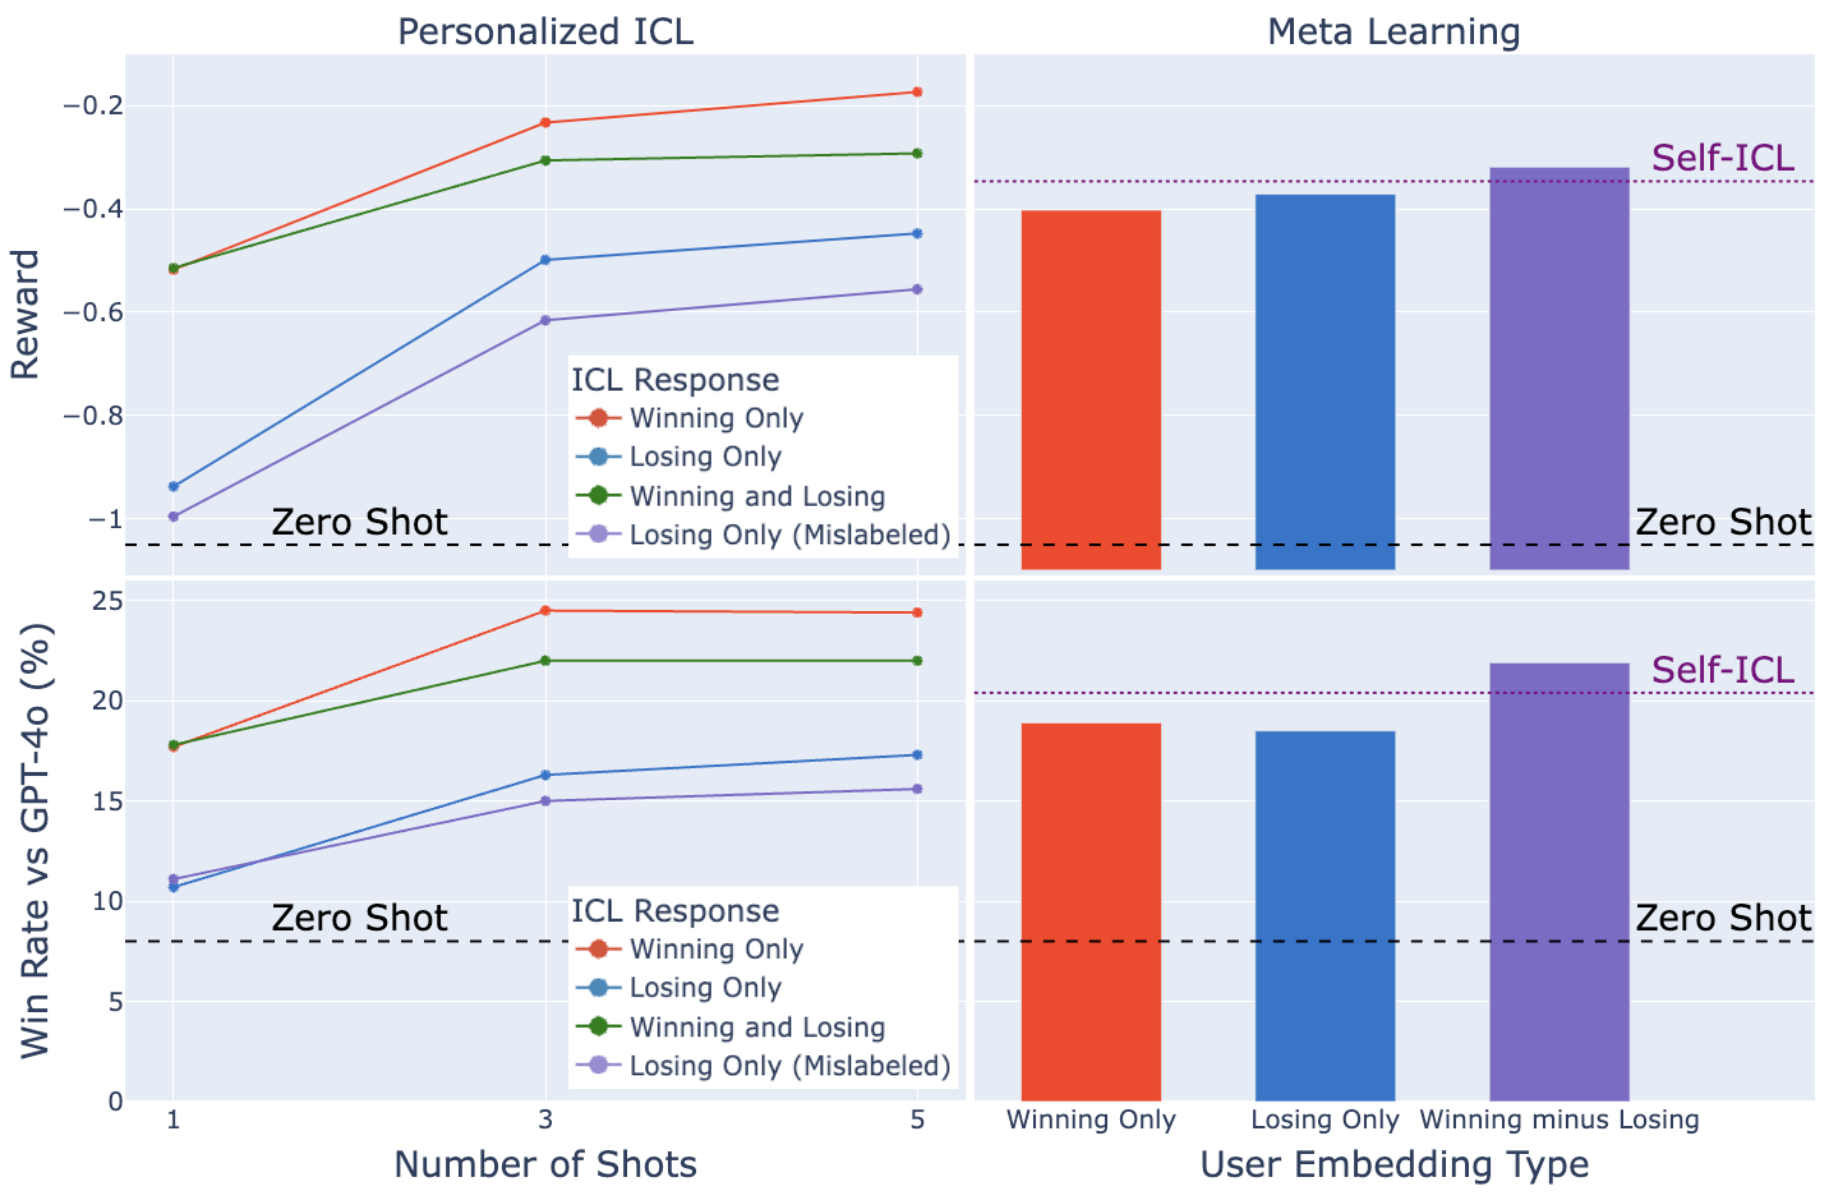
\includegraphics[width=\textwidth]{figures/fig6sharp.png}
    \caption{Results across different personalization algorithms. 
    \textbf{(Left)} Test users are accompanied by a relevant interaction history with pairwise preference feedback, and we explore the LLM's ability to exploit this information in context. 
    \textbf{(Right)} Test users have interaction histories that are not relevant to their test prompt, and we probe methods for embedding users based on language feedback to retrieve useful examples from simular users for ICL.}
    \label{fig:exp_results}
\end{figure}


\subsection{Learning Across Users}

Having established some empirical foundations for in-context personalization with \textsf{PersonalLLM}, we next highlight a particularly significant challenge prevalent in practice that has been under-explored in the LLM community: the cold-start problem. 
When a new user with limited prior interaction data arrives, or a user inquires about a new topic, prior user interactions alone cannot inform a satisfactory response.
We model this challenge as a meta-learning problem, where the goal is to utilize a rich reservoir of prior interactions with a diverse set of users. 
We are motivated by real-world scenarios where we have access to a proprietary database containing extensive interaction histories from previous users. 
When a new user arrives, our goal is to utilize this rich, heterogeneous dataset to provide the best possible response to the new user's query despite having only limited initial interactions with them that may not be relevant to the current query. 
This setting resembles typical recommendation systems, but "actions" are now defined over the space of natural language outputs instead of a fixed set of items.
See Figure~\ref{fig:metalearn} for further illustration.

Our experiment explores the open question of how best to embed (e.g., represent with some vector) users based on small amounts of natural language feedback.  
With effective algorithms to lookup similar users, more relevant interactions may be leveraged to improve a response to a new user query.
While a rich literature exists on information retrieval (i.e., RAG) for typical NLP benchmark tasks like question answering and fact checking \citep{lewis2021retrievalaugmentedgenerationknowledgeintensivenlp, gao2024retrievalaugmentedgenerationlargelanguage}, the distinctive nature of the personalization task necessitates new algorithms.

\subsubsection{Experiment Details}

For each of our 1,000 test users, we build a short but, in contrast to our first experiment, \textit{possibly irrelevant} interaction history by retrieving 5 random prompts.  Winning/losing response pairs (i.e., preference feedback) are selected as before.  In order to supplement these interaction histories, we sample a historical database of 10,000 users (also with $\alpha=0.05$), each with a set of 50 prompt, winning response, losing response triplets from the train set, where the prompts are selected randomly and the winning and losing responses are selected as the historical user's highest and lowest scoring among the 8.

We compare 3 methods for embedding users for lookup:
\begin{itemize}
    \item \textbf{Winning minus Losing:} Average direction in embedding space between winning and losing responses for each prompt.
    \item \textbf{Winning only:} Average direction in embedding space for winning responses. 
    \item \textbf{Losing only:} Average direction in embedding space for losing responses.
\end{itemize}

For each test user, we build a set of candidate prompt/feedback data by retrieving the 20 most similar historical users based on cosine similarity of their embeddings, and then of the pool created by those users' interaction histories, retrieving 3 examples for in-context learning based on prompt embedding similarity to the user's test prompt.  We compare to a \textbf{Self-ICL} baseline, where the test user's possibly irrelevant prompt/feedback history is used for ICL.  Evaluation is done as before.

\subsubsection{Results}

Our results are shown in Figure~\ref{fig:exp_results}.  
We find that using the strongest user embedding method, which most fully exploits the available pairwise preference feedback, meta-learning can beat the self-ICL baseline.
This positive result for meta-learning highlights the opportunity created by leveraging historical user data, and the feasibility of embedding users based on a small amount of language feedback.
However, the gain from our relatively naive method is small, illustrating the need for methodological innovation in building such systems.
